\chapter{C\lowercase{ase} S\lowercase{tudies}}


\section{Introduction}
In this chapter we provide a more detailed discussion on how to apply the learning algorithm we have been developing to a given problem. Firstly, we shall provide some general guidelines for tuning the learning control approach. This will be followed by a comparison of our method with a standard control theoretic approach to the same problem. These comparisons will consist of a discussion regarding the entire design process from beginning to end and the component parts involved. We aim to provide insight into the advantages and disadvantages associated with applying each methodology, as a non-expert, to a given problem. The case studies we investigate are the unicycle control problem, introduced in \Sec{unicycle}, and a simulated process control problem: the evaporator.
%
As we have already discussed the unicycle control task we shall give this problem less attention than the evaporator. With the evaporator we additionally aim to demonstrate the power of the learning control approach in two ways: the ability to learn more exotic control policies than a standard affine structure and to demonstrate a level of robustness in the face of erroneous prior information.





\section{Guidelines for Tuning}
We begin this chapter with a breakdown of the elements of the learning algorithm that need to be chosen a priori and some guidelines for how to choose or initialise them.
\begin{itemize}
\item
{\bf Prior Over Dynamics.} Choosing an appropriate prior over dynamics functions is one of the most involved aspects of setting up the algorithm. It can be broken up as follows:
\begin{itemize}
\item
\textit{State Representation.} This is, in general, a difficult question in which we usually rely on domain specific knowledge of the problem in order to define the state. Once we have the state we need to determine how to map the current state and action to the next state. We usually do this in two stages: predict the difference between the next and current state using a zero mean Gaussian process prior then reconstruct the next state from this prediction.
\item
\textit{Known Relationships.} If there are known relationships between a subset of the state variables these can be included directly using the framework of Chapter 4.
\item
\textit{Angular Variables.} These can be dealt with using  a sine/cosine representation of the angle at the input to the GP model which can then be reconstructed at the next timestep using simple linear and trigonometric relationships.
\item
\textit{Hyperparameters.}  To initialise the length-scale and output variance hyperparameters of a standard squared exponential kernel a good starting place is to set them to the standard deviations of the input and output training data sets respectively.
\item
\textit{Pseudo-Inputs.} The number of pseudo-inputs used when sparse approximations are employed depends on how much computational saving is required. For the unicycle problem we found that 300 was more than ample to capture all salient features. The locations were initialised as a random subset of the full training data set.
\end{itemize}
\item
{\bf Cost Function.} As discussed in \Sec{natexp}, an appropriate form of stage-cost is the inverted-Gaussian as it has useful properties in terms of the exploration-exploitation tradeoff. The width of this stage-cost should be chosen in such a way as to cover the ``normal" region of operation of the system, so that the gradients involved in the optimization stage are not negligible. The prediction horizon should be set as long as possible under the computational constraints of the offline simulation phase.
\item
{\bf Policy Structure.}
The rule of thumb we use when picking a policy structure is to be as simple as possible. As we increase the complexity from a standard affine structure to a that of a radial basis function there can be a huge increase in the number of parameters that need to be optimised, therefore a larger space to search for a control solution and a potential increase of local optima. However, for some problems a nonlinear policy structure is necessary e.g.\ the pendulum swing-up task.
\item
{\bf Sampling Time.} The sampling time should be chosen as long enough such that the computation in the prediction, or evaluation, phase is as low as possible but short enough for the control task to be achievable. This can be a tricky parameter to tune. For example, if we used a value of 0.2$\,$s for the unicycle then the control task appeared to be impossible, but a value of 0.1$\,$s led to impractical computation time.
\item
{\bf Interaction Phase.}
The goal of the interaction phase is to run the current control policy long enough to capture useful new information but not long enough so that the training data set gets too big too quickly. Again, the upper limit is controlled by the computational complexity of the simulation phase. An example of one heuristic we used to determine this run-time for the unicycle example is given in \Sec{unicycle}.
\item
{\bf Simulation Phase.}
A final important parameter is the number of function evaluations, or line searches, we limit the gradient descent optimisation scheme to. One rule of thumb when choosing this parameter is that in a standard conjugate gradient scheme it takes around the same number of function evaluations as there are policy parameters to be optimised in order to reach a reasonable approximation of the Hessian matrix. Therefore, setting the number of function evaluations to at least twice this number worked well in the problems we tackled.
\end{itemize}

With these tuning rules in mind we shall now move onto the case studies themselves to gain some further practical insight into this method.

%In order to help visualise all the steps involved in applying the algorithm we refer to the pseudo-code given in Algorithm~\ref{alg:learn}.


%\begin{algorithm}[]
%\small
%\SetAlgoLined
%\KwData{Initial training data set $\cD_0$, initial control policy $\bpi_0$, prior over dynamics $p(\bff)$, cost function $J(\cdot)$, sampling time $\Dt$, starting state $p(\bx_0)$}
%\KwResult{A working control policy $\bpi$}
%$i = 0$ \;
%Augment the state distribution $p(\bx_i)$ with the sines/cosines of angle variables to give $p(\bar\bx_i)$ \tcc*{SIMULATION}
%Append the control actions to find $p(\bar\bz_i)$ using $p(\bar\bx_i)$ and the current policy $\bpi_i$ \;
%
%Evaluate the stage cost
%
%\For{$j=1 \to N$}
%eggs\;
%\EndFor
%\caption{Pseudo-code for the different phases of the learning algorithm. Note that $N$ is the maximum number of }
%\label{alg:learn}
%\end{algorithm}





\section{Unicycle}
\subsection{Problem Overview}
We shall now discuss the issues involved in learning control policies for the unicycle problem we outlined in \Sec{unicycle}. For ease of reference we include the figure from \Sec{unicycle} again here, in \Fig{uniboy}. Remember that the only control actions we may apply are a torque on the wheel $u_{\te{w}}$ and a torque on the turntable at the top of the unicycle $u_{\te{t}}$. Therefore we do not have any direct control of the rolling motion $\theta$, which makes the control task intrinsically difficult. In order to understand more fully the difficulty of this control problem we begin with working through a procedure of how to apply standard linear control theory to the problem. This will be followed by a discussion of the associated issues with applying our learning algorithm. We note that all the following analysis is carried out with respect to the nonlinear equations of motion derived by \cite{For09}. These equations and their derivation are given a full treatment in \App{unicycle}.




%-------------------------------------------------------------------------------------------------------------------------------------------
\begin{figure}[t]
\centering
\input{figs/apps/unicoords_body}
\caption{The robotic unicycle. The spatial position of the unicycle is defined by the pitch angle $\phi$, roll angle $\theta$, yaw angle $\psi$, wheel angle $\phi_\te{w}$, turntable angle $\psi_\te{t}$ and the body-centred coordinates of the global origin $(x_\te{c},y_\te{c})$. The controlled inputs are the motor torque applied to the wheel $u_\te{w}$ and the motor torque applied to the turntable $u_\te{t}$.}
\label{fig:uniboy}
\end{figure}
%-------------------------------------------------------------------------------------------------------------------------------------------



\subsection{Linear Control Theory}
\subsubsection{Linearised Model Selection}

From a standard control theory perspective, the first step towards designing a stabilising policy is usually to obtain a linear model of the system which describes the dynamics in the region of some operating point $\bar\bz$ in the state-action space. Recall that for the unicycle, the state is given by $\bx = [\phi, \dot\phi, \theta, \dot\theta, \psi, \dot\psi, \dot\phi_\te{w}, \dot\psi_\text{t},x_\text{c}, y_\text{c}]^\top \in \RR^{10}$ with pitch angle $\phi$, roll angle $\theta$, yaw angle $\psi$, wheel angle $\phi_\te{w}$, turntable angle $\psi_\te{t}$ and the location of the origin $(x_\te{c},y_\te{c})$ with respect to a body-fixed reference frame. These are depicted in \Fig{uniboy}. 

A reasonable state-action location around which to find a linearised model of the system is $\bar\bz = \bO$. In this state the unicycle is stationary and upright. To obtain a linearised model of the form $\dot\bx = \bA\bx + \bB\bu$ from the full nonlinear equations $\dot\bx = \bff(\bx,\bu)$ we apply the following procedure of numerical integration to get the columns of the $\bA$ and $\bB$ matrices
\begin{align*}
A[:,i] &= \Big( \bff(\bar\bx+\epsilon\bee_i,\bar\bu) - \bff(\bar\bx-\epsilon\bee_i,\bar\bu) \Big)/2\epsilon, i\in \ZZ_{[1,E]} \\
B[:,j] &= \Big( \bff(\bar\bx,\bar\bu+\epsilon\bee_j) - \bff(\bar\bx,\bar\bu-\epsilon\bee_j) \Big)/2\epsilon, j\in \ZZ_{[1,F]}
\end{align*}
where $\epsilon$ is some small scalar perturbation and $\bee_i$ is the $i\tth$ column of the identity matrix of appropriate dimensions. Applied to the unicycle equations and using $\epsilon = 10^{-6}$ leads to the linearised state space system
\begin{equation*}
\underbrace{
\bmat{  \dot\phi \\ \ddot\phi \\ \dot\theta \\ \ddot\theta \\ \dot\psi \\ \ddot\psi \\ \ddot\phi_\te{w} \\ \ddot\psi_\te{t} \\ \dot x_\te{c} \\  \dot y_\te{c}  } 
}_{\dot\bx }
= 
\underbrace{
\bmat{
\cdot  &  1 & \cdot & \cdot & \cdot  &  \cdot & \cdot & \cdot & \cdot & \cdot \\
79.4  &  \cdot & \cdot & \cdot & \cdot &  \cdot & \cdot & \cdot & \cdot & \cdot \\
\cdot  &  \cdot & \cdot & 1 & \cdot  & \cdot & \cdot & \cdot & \cdot & \cdot \\
\cdot  &  \cdot & 10.7 & \cdot & \cdot  & \cdot & \cdot & \cdot & \cdot & \cdot \\
\cdot  &  \cdot & \cdot & \cdot & 1  & \cdot & \cdot & \cdot & \cdot & \cdot \\
\cdot  &  \cdot & \cdot & \cdot & \cdot  & \cdot & \cdot & \cdot & \cdot & \cdot \\
-207  &  \cdot & \cdot & \cdot & \cdot  & \cdot & \cdot & \cdot & \cdot & \cdot \\
\cdot  &  \cdot & \cdot & \cdot & \cdot  & \cdot & \cdot & \cdot & \cdot & \cdot \\
\cdot  &  \cdot & \cdot & \cdot & \cdot  & \cdot & -0.225 & \cdot & \cdot & \cdot \\
\cdot  &  \cdot & \cdot & \cdot & \cdot  & \cdot & \cdot & \cdot & \cdot & \cdot 
}
}_{\bA}
\underbrace{
\bmat{  \phi \\ \dot\phi \\ \theta \\ \dot\theta \\ \psi \\ \dot\psi \\ \dot\phi_\te{w} \\ \dot\psi_\te{t} \\ x_\te{c} \\  y_\te{c}  } 
}_{\bx}
+ 
\underbrace{
\bmat{
\cdot & \cdot \\
\cdot & -1.40 \\
\cdot & \cdot \\
\cdot  &  \cdot \\
\cdot  &  \cdot \\
-2.23 &  \cdot \\
\cdot & 4.21 \\
7.23 & \cdot \\
\cdot  & \cdot \\
\cdot  & \cdot
}
}_{\bB}
\underbrace{
\bmat{u_{\te{w}} \\ u_{\te{t}}}
}_{\bu}
\end{equation*}
where the dots indicate zero terms. It is clear from inspection that this is an uncontrollable system of equations. In particular, we cannot control the roll angle $\theta$ or the velocity $\dot\theta$ since they are independent of the rest of the dynamics and cannot be influenced directly through the available actuators. This would be ok if they formed a stable sub-system, however this is clearly not the case. To see why, consider a small positive perturbation of $\theta$ from its equilibrium, this leads to a positive acceleration through the 10.7 term and therefore $\theta$ will continue to increase in an unbounded fashion. In other words, the unicycle will fall over.

%where the $a_i$s and $b_i$s are non-zero constants and the dots indicate zeros. The condition for controllability is that the controllability matrix $\mathcal{C} = \big[\bB, \bA\bB \dots \bA^{E-1}\bB\big]$ has full row rank. For this system however $\mathrm{rank}(\mathcal{C}) = 5$ meaning there are four uncontrollable modes. It is still possible that the system is stabilisiable if each of these modes is stable. To find out what these modes are consider the left null-space of $\mathcal{C}$ which in this case is spanned by the following orthogonal bases
%\begin{equation*}
%\mathrm{null}\big(\mathcal{C}\T\big)= \bmat{
%\cdot  & 1 & \cdot & \cdot \\
%\cdot  & \cdot & c_1 & c_2 \\
%\cdot  & \cdot & \cdot & \cdot \\
%\cdot  & \cdot & \cdot & \cdot \\
%\cdot  & \cdot & \cdot & \cdot \\
%\cdot  & \cdot & \cdot & \cdot \\
%1  & \cdot & \cdot & \cdot  \\
%\cdot  & \cdot & c_3c_5 & c_3c_6 \\
%\cdot  & \cdot & c_4c_5 & c_4c_6 
%}
%\end{equation*}
%for some more non-zero constants $c_i$. Unfortunately the second, third and fourth modes here are unstable while the mode associated with $y_\text{c}$ is an integrator. This is an especially bad situation since the roll angle $\theta$ is uncontrollable. 
From the above analysis we evidently require a different operating point in order to find a stabilisable linear system. From inspection of the nonlinear equations of motion, found in \App{unicycle}, we can observe that the rotational motion governed by $\psi, \dot\psi, \dot\psi_\te{t}$ and $u_\te{t}$ is decoupled from the other states when the unicycle is upright i.e.\ $\theta = \phi = 0$. This linearised subsystem is governed by the integrator equations
\begin{equation*}
\bmat{\dot\psi \\ \ddot\psi \\ \ddot\psi_\te{t}} = 
\bmat{0 & 1 & 0 \\ 0 & 0 & 0 \\ 0 & 0 & 0}
\bmat{\psi \\ \dot\psi \\ \dot\psi_\te{t}}
+
\bmat{0 \\ -2.23 \\ 7.23} \bmat{ u_\te{t} }
\end{equation*}
We could then set the unicycle spinning at some constant velocity by applying some pulse action through $u_{\text{t}}$. For example, applying $u_{\text{t}}=10\,$N$\,$m for 0.1$\,$s would lead to $\dot\psi = -2.23\,$rad$\,$s$\inv$ and $\dot\psi_{\te{t}} = 7.23\,$rad$\,$s$\inv$. Note that this system is only controllable along a single dimension of the two dimensional space. Now if we linearised around this operating point the other states would be governed by the following system of equations
\begin{equation}
\underbrace{
\bmat{  \dot\phi \\ \ddot\phi \\ \dot\theta \\ \ddot\theta \\ \ddot\phi_\te{w} \\ \dot x_\te{c} \\  \dot y_\te{c} }
}_{\dot\bx_{\te{rot}}}
=
\underbrace{ \bmat{
\cdot  &  1 & \cdot & \cdot & \cdot  &  \cdot & \cdot \\
85.2  &  \cdot & \cdot & -4.94 & \cdot &  \cdot & \cdot \\
\cdot  &  \cdot & \cdot & 1 & \cdot  & \cdot & \cdot \\
\cdot  &  3.40 & 15.7 & \cdot & 0.548  & \cdot & \cdot \\
-209  &  \cdot & \cdot & -3.12 & \cdot  & \cdot & \cdot \\
\cdot  &  \cdot & \cdot & \cdot & -0.225  & \cdot & -2.23 \\
\cdot  &  \cdot & \cdot & \cdot & \cdot  & 2.23 & \cdot 
}
}_{\bA_{\te{rot}}}
\underbrace{
\bmat{  \phi \\ \dot\phi \\ \theta \\ \dot\theta  \\ \dot\phi_\te{w}  \\ x_\te{c} \\  y_\te{c}  } 
}_{\bx_{\te{rot}}}
+
\underbrace{ \bmat{
\cdot \\
-1.40 \\
\cdot \\
\cdot \\
4.21 \\
\cdot \\
\cdot
}
}_{\bB_{\te{rot}}}
\bmat{u_{\te{w}} }
\label{eqn:LQmodel}
\end{equation}
To investigate the controllability of this new system of equations we evaluated the controllability matrix $\mathcal{C} = \big[\bB_{\te{rot}}, \bA_{\te{rot}}\bB_{\te{rot}}, \dots, \bA_{\te{rot}}^{6}\bB_{\te{rot}}\big]$. The condition for controllability is that this matrix has full row rank, and means that there exists a set of actions that can force the system into any part of the state space. This new system leads to a controllability matrix with full rank and can therefore be used in the design of a control policy for this subset of state variables. The turntable torque would simply be used to maintain the rotational equilibrium values. It is worth noting that although, in this linear model, the rotational dynamics are decoupled from the rest of the dynamics, the rotational setpoint values for $\dot\psi$ and $\dot\psi_{\te{t}}$ will still affect the constants in the $\bA_{\te{rot}}$ matrix.




%As can be seen this spinning setpoint produces a new set of non-zero constants $d_i$ in the $\bA$ matrix (with the exception of $a_4$) which in turn produces a controllability matrix with $\mathrm{rank}(\mathcal{C}) = 8$. The single uncontrollable mode is due to the rotational dynamics that have already been discussed. It is clear then from this linearised model that the rotational dynamics of the unicycle are still completely decoupled from the other dynamics and can therefore be treated separately. The only requirement for $u_{\te{t}}$ then is to pulse the angular velocities $\psi$ and $\psi_{\te{t}}$ into their setpoint values. Given this single requirement for the turntable the other dynamics can now be treated separately using the fully controllable state space $\bx_{\mathcal{C}} = [\theta, \dot\theta, \phi, \dot\phi, \dot\psi_\text{w}, x_\te{c}, y_\te{c}]^\top \in \RR^{7}$ with dynamics
%
%which is now in a form amenable to standard linear control theoretic results. It is worth noting that although the rotational dynamics are decoupled from the rest of the dynamics in this linearised form, the rotational setpoint values for $\psi$ and $\psi_{\te{t}}$ will still affect the $d_i$ values and therefore need to be taken into consideration.


The process of finding an appropriate linear model to use as the basis for standard control methods clearly requires a relatively in depth knowledge of the dynamic equations governing the system. We would like to make the additional point that in this study the solution of linearising around a spinning trajectory came about when we considered the control policy obtained by our learning algorithm! The learned solution would always rotate on the spot instead of coming to a complete rest and it was actually this behaviour that pointed us to analyse the nonlinear equations to find a controllable form.


\subsubsection{Policy Design}
Now that a suitable linear model has been obtained we can think about control policy design. There is a plethora of multivariable linear control design methodologies available to us at this stage. Let us consider the commonly used Linear Quadratic Regulator (LQR) approach to the problem. The discrete-time LQR is the solution to the following optimisation problem
\begin{align}
& \text{minimise} & J =  & \sum_{k=0}^{H}  \bx_k\T\bQ\bx_k + \bu_k\T\bR\bu_k && \label{eqn:lqr1} \\
&\text{subject to} & \bx_{k} &= \bA\bx_{k-1} + \bB\bu_{k-1} && \label{eqn:lqr2}
\end{align}
for some suitable quadratic cost function parameterised by the matrices $\bQ$ and $\bR$. The optimal solution turns out to be a causal, linear control law $\bpi$ which is dependant only on the current state and may be calculated in closed form, even for the infinite horizon, $H \rightarrow \infty$, case. This problem and its solution appeared in the seminal paper by \cite{Kal60b}. The only design choice in this case is how to choose the $\bQ$ and $\bR$ matrices. This is generally a heuristic process since we need to tune these parameters in order to create a policy which addresses
\begin{itemize}
\item {\bf Performance:} by which we mean that the policy can actually achieve the task it was designed for
\item {\bf Constraints:} ensures that state and action constraints are not violated under ``normal" operating conditions
\item {\bf Model Mismatch:} the policy must achieve the control task under the knowledge that the actual system may be significantly different
\end{itemize}
Ideally we would like to decouple these requirements and address them individually rather than simultaneously through a given set of parameters. This can be done in a variety of ways which we shall now discuss. %Consider instead the framework of $\mathcal{H}_\infty$ loop-shaping. This can formally address model mismatch by pulling out the uncertain elements in the transfer functions and placing hard bounds on where they will lie. This process, however, will require careful tuning and estimation of the uncertainty bounds.
%


One way to separate the problem of constraint violation from the stage cost is to use Model Predictive Control (MPC). In a standard MPC algorithm we do not find a closed form for the feedback policy $\bpi$ but instead perform a constrained version of \Eqs{lqr1}{lqr2} online over the future action sequence $\{\bu_0\dots\bu_H\}$. We then apply the first action in this optimal sequence and repeat the procedure at the following timestep. Obviously this is more computationally intensive in terms of online operation. However, if the constraints are linear then this forms a quadratic programming problem which is convex and there exist fast and efficient algorithms for solving such problems e.g.\ \cite{BoVa04}.




Addressing the issue of model mismatch in the third bullet point is a more difficult issue. Methods from the field of Robust Control can tackle this issue by defining a nominal system and considering a bounded set of perturbations from this system. Control policies can then be derived which will satisfy some stability and/or performance criteria across all possible systems in the set. We note that determining an appropriate set of perturbed models can be a difficult problem.

Another common approach, instead of using a single linearised model and perturbations around it, is to find linearisations around a few operating points, solve the given LQR problem at each operating point and then smooth, or switch, between the solutions when applying them online. This is known as Gain Scheduling. How to choose the operating points and the smoothing function are of course heuristic problems. 
%
Alternatively, re-linearisation could be done in an adaptive manner online in the spirit of the self-tuning regulator except that the new model need not be based on the observed data but a linearisation of an internal nonlinear one. Again, an issue with this would be how we could guarantee the feasibility of the resulting solution. In our example of the unicycle, how do we guarantee that the linearised system is actually controllable?

We now turn to the problem of choosing a suitable sampling time $\Dt$. The only constraint in the case of LQR is the speed at which the feedback policy can be evaluated, which will be very fast indeed since it will simply be a single matrix multiplication. For MPC this will be more of a bottleneck since a full optimisation program needs to be solved at each timestep. However, if the problem is a quadratic program then for a problem the size of the unicycle modern algorithms should be able solve it on the order of 0.01 to 0.001$\,$s and therefore should not be a problem in this case.


\subsection{Learning Control}
We now consider the design process for the learning algorithm we have proposed in previous chapters.  The major design choices available here are the form of the stage cost $c$, the sampling time $\Dt$ and the form of prior over the unknown dynamics. Since this framework makes only high level assumptions regarding the form of the dynamics and it naturally incorporates modelling uncertainty the problem of model-system mismatch has been rigorously addressed. Furthermore, action constraints can be dealt with in the manner outlined in \Sec{actioncon}. Therefore we need only use our stage-cost to encode the performance criteria.

For the case of learning a policy to balance the unicycle we can simply define a quadratic stage-cost that penalises the squared Euclidean distance of the top of the unicycle to the upright position at the origin. This is a very intuitive form of cost. However, as we discussed in \Sec{natexp}, the quadratic stage cost may not be conducive for learning control. Therefore we use a saturated quadratic (or inverted-Gaussian) stage cost. The remaining free parameters are then to do with the width of this cost. Again, a natural choice would be to choose the two standard deviation region to cover the likely ``area of operation".  In practice, this intuitive choice of cost had to be tuned slightly to penalise deviation in the vertical direction more heavily to encode the notion that falling over is a more costly mistake than not being in the right location.


The second issue is how to choose the sampling time $\Dt$. In this instance the sampling time is very much a bottleneck of the algorithm. In order to keep the offline policy optimisations in the order of hours rather than days we were constrained to choose sampling times greater than $0.1\,$s. However, beyond $0.2\,$s the control problem becomes too difficult and our algorithm cannot find a stabilising policy using this sampling time. We emphasise that this is not a problem for the online implementation (which is simply a linear policy) but for the offline optimisation.


One of the major advantages of this data-driven approach is that we avoid many of the problems associated with using a first-principles model of the system. Attacking the problem using a first-principles model will inevitably require much more expert-knowledge on the dynamics of the system at hand and a good understanding of which particular physical assumptions are likely to be poor. The data-driven approach moves many of the assumptions to a more conceptual level and therefore the domain-specific knowledge required in terms of modelling is greatly reduced.



\subsection{Comparison of the LQR and Learned Policies}
We now provide a brief comparison of the performance and policy structures obtained by the LQR approach and the learning approach outlined in the previous sections. To aid in a direct comparison we chose $\Dt = 0.15\,$s as the sampling time for the LQR policy. To obtain the LQR policy we chose a spinning operating point of $\dot\psi = -2.23\,$rad$\,$s$\inv$ and $\dot\psi_{\te{t}} = 7.23\,$rad$\,$s$\inv$ and all other states at the origin. This gave us the linear model in \Eq{LQmodel}. A simple affine control policy mapping $\dot\psi$ to $u_\te{t}$ was then designed (using LQR with a state weight of 1 and action weight of 0.1) to regulate the spinning motion.

The next step is to design an LQR policy for the other states and actions. We then chose the state weighting matrix $\bQ$ to penalise the squared distance of the top of the unicycle to the upright position over the origin, similar to how we chose the stage-cost for the learning algorithm in \Eq{unicost}. This gives us
\begin{align*}
\bx_{\te{rot}}\T\bQ\bx_{\te{rot}} &= \big(x_\te{c} - r\phi\big)^2 + \big(y_\te{c} - (r+r_\te{w})\theta\big)^2 \\
&\approx \big(x_\te{c} - r\sin\phi\big)^2 + \big(y_\te{c} - (r+r_\te{w})\sin\theta\big)^2
+ \big( (r+r_\te{w}) - (r_\te{w} + r\cos\phi)\cos\theta \big)^2
\end{align*}
for $\phi$ and $\theta \approx 0$. As before, $r$ is the unicycle frame length and $r_\te{w}$ is the radius of the wheel. We then tuned $R$ by gradually increasing it from zero until the resulting control policy was stabilising. As a result of this procedure we chose $R = 0.001$.



% ------------------------------------------------------------------------------------------------------------------------
\begin{figure}
\centering
\footnotesize
\subfigure[\footnotesize Pitch $\phi$]{\includegraphics[scale=0.63]{figs/comp/unirun_LQ1.pdf}}
\subfigure[\footnotesize Roll $\theta$]{\includegraphics[scale=0.63]{figs/comp/unirun_LQ2.pdf}}
\subfigure[\footnotesize Yaw $\psi$]{\includegraphics[scale=0.63]{figs/comp/unirun_LQ3.pdf}}
\subfigure[\footnotesize Location $x_\te{c}$]{\includegraphics[scale=0.63]{figs/comp/unirun_LQ4.pdf}}
\subfigure[\footnotesize Location $y_\te{c}$]{\includegraphics[scale=0.63]{figs/comp/unirun_LQ5.pdf}}
%
\subfigure[\footnotesize Pitch $\dot\phi$]{\includegraphics[scale=0.63]{figs/comp/unirun_LQ6.pdf}}
\subfigure[\footnotesize Roll $\dot\theta$]{\includegraphics[scale=0.63]{figs/comp/unirun_LQ7.pdf}}
\subfigure[\footnotesize Yaw $\dot\psi$]{\includegraphics[scale=0.63]{figs/comp/unirun_LQ8.pdf}}
\subfigure[\footnotesize Wheel $\dot\phi_\te{w}$]{\includegraphics[scale=0.63]{figs/comp/unirun_LQ9.pdf}}
\subfigure[\footnotesize Turntable $\dot\psi_\te{t}$]{\includegraphics[scale=0.63]{figs/comp/unirun_LQ10.pdf}}
\caption{State trajectories over 10$\,$s of the unicycle when an LQR policy is applied in order to move from the initial position $(x_\te{c},y_\te{c}) = (0,1)$ to the origin. The policy is derived from a linear model obtained from a spinning operating point. The values of this operating point for each state are shown in red, and dashed lines for the spinning states $\dot\psi$ and $\dot\psi_\te{t}$.}
\label{fig:LQuni}
\end{figure}
% ------------------------------------------------------------------------------------------------------------------------



The result of applying this LQR control policy to the unicycle for the task of moving from a starting position $(x_\te{c},y_\te{c}) = (0,1)$ to the origin is shown in \Fig{LQuni}. We can see that the control policy is quite aggressive but converges to the spinning operating point within 4\,s. Further tuning, could of course improve this performance but will not be pursued further here.
%
The result of applying one of the learned control policies from \Sec{unicycle} is shown in \Fig{MLuni}. In this case, the trajectory it follows converges on a tight circular orbit, with a radius of around $20\,$cm and a roll angle of $0.1\,$rad, rather than spinning exactly on the origin. This solution was found the vast majority of the time when using this cost function. We note that this trajectory does not appear to be much worse in terms of stage-cost since the values $(x_\te{c}, y_\te{c}) = (0,0.2)\,$m and $\theta = 0.1\,$rad yield a very small stage-cost of around 0.005. This simply highlights the issue that it is often hard to design an intuitive cost that produces a good control policy. 




% ------------------------------------------------------------------------------------------------------------------------
\begin{figure}
\centering
\footnotesize
\subfigure[\footnotesize Pitch $\phi$]{\includegraphics[scale=0.63]{figs/comp/unirun_ML1.pdf}}
\subfigure[\footnotesize Roll $\theta$]{\includegraphics[scale=0.63]{figs/comp/unirun_ML2.pdf}}
\subfigure[\footnotesize Yaw $\psi$]{\includegraphics[scale=0.63]{figs/comp/unirun_ML3.pdf}}
\subfigure[\footnotesize Location $x_\te{c}$]{\includegraphics[scale=0.63]{figs/comp/unirun_ML4.pdf}}
\subfigure[\footnotesize Location $y_\te{c}$]{\includegraphics[scale=0.63]{figs/comp/unirun_ML5.pdf}}
%
\subfigure[\footnotesize Pitch $\dot\phi$]{\includegraphics[scale=0.63]{figs/comp/unirun_ML6.pdf}}
\subfigure[\footnotesize Roll $\dot\theta$]{\includegraphics[scale=0.63]{figs/comp/unirun_ML7.pdf}}
\subfigure[\footnotesize Yaw $\dot\psi$]{\includegraphics[scale=0.63]{figs/comp/unirun_ML8.pdf}}
\subfigure[\footnotesize Wheel $\dot\phi_\te{w}$]{\includegraphics[scale=0.63]{figs/comp/unirun_ML9.pdf}}
\subfigure[\footnotesize Turntable $\dot\psi_\te{t}$]{\includegraphics[scale=0.63]{figs/comp/unirun_ML10.pdf}}
\caption{State trajectories over 10$\,$s of the unicycle when a learned affine policy is applied in order to move from the initial position $(x_\te{c},y_\te{c}) = (0,1)$ to the origin. The values of the operating point used for the LQR policy, from \Fig{LQuni}, for each state are shown in red, and dashed lines for the spinning states $\dot\psi$ and $\dot\psi_\te{t}$.}
\label{fig:MLuni}
\end{figure}
% ------------------------------------------------------------------------------------------------------------------------



Finally, the resulting policy gain matrices produced by the LQR and learning methods are
\begin{align*}
\bK_1\T &= \bmat{
73.4 & 0 \\
20.7 & 0 \\
-125 & 0 \\
-21.78 & 0 \\
0 &  0 \\
0 & 1.91 \\
3.54 & 0   \\
0  & 0 \\
 -2.82 & 0 \\
 4.43 & 0 
} &
%
\bK_2\T &= \bmat{
79.8 & -4.18 \\
11.8 &  4.51 \\
26.9 & -93.7 \\
1.31 & -28.7 \\
0.08 & -0.09  \\
-3.35 & 4.72 \\
1.15 &  0.98 \\
-0.69 &  0.90 \\
-4.37 &  1.15 \\
-3.09 &  4.08 \\
} 
%
%\\ L_{LQ}\T &= \bmat{-4.24 & 0} &
%
%L_{ML}\T &= \bmat{1.82 & -3.00} 
\end{align*}
respectively. Note that the columns of the gain matrices (rows of the transposed matrices) correspond to elements of the state vector $\bx = [\phi, \dot\phi, \theta, \dot\theta, \psi, \dot\psi, \dot\phi_\te{w}, \dot\psi_\text{t},x_\text{c}, y_\text{c}]^\top$. We can observe that the learning algorithm has utilised all the states available to it as feedback terms whereas, due to the way we structured the problem the LQ policy is sparse. We also note an issue with the the learned gain matrix $\bK_2$. Since there are non-zero feedback gains on the yaw angle $\psi$, the orbital trajectory will not go on indefinitely since these feedback terms will begin to dominate the control actions (in fact the unicycle falls over at around 30$\,$s). However, since this is not an issue over the ten second horizon it is not picked up by the algorithm. This is an example of one of the potential issues with optimising over a finite prediction horizon.







\section{Process Control} %%%%%%%%%%%%%%%%%%%%%%%%%%%%%%%%%%%%%%%


\subsection{Problem Overview}
We now consider a significantly different control problem, that of a forced-circulation industrial evaporator as outlined by \cite{NeLe89} and depicted in \Fig{evap}. This problem was used to demonstrate the capabilities of nonlinear MPC in \cite{Mac02}. The full equations of motion and values for the physical constants can be found in \App{evaporator}.

The system works as follows: a feed stream enters the system with concentration $X_1$, temperature $T_1$ and flow rate $F_1$. This is mixed with recirculating liquid and is pumped through the evaporator at a flow rate $F_3$. The evaporator is a heat exchanger with internal pressure $P_2$ and is heated by steam with flow rate $F_{100}$, pressure $P_{100}$ and temperature $T_{100}$. The feed and recirculated liquid is boiled inside the evaporator and the resulting mixture of vapour and liquid enters the separator with liquid level $L_2$. A small proportion of the liquid from the separator is drawn off as product, with concentration $X_2$, temperature $T_2$ at flow rate $F_2$. The vapour drawn off from the separator flows to a condenser at flow rate $F_4$ and temperature $T_3$ where it is condensed by cooling water with flow rate $F_{200}$, entry temperature $T_{200}$ and exit temperature $T_{201}$.




This system has three states consisting of the product composition $X_2$, the evaporator pressure $P_2$ and the separator level $L_2$. The choice of these states is clear when we consider the equations in \App{evaporator}. The control actions are chosen to be the product flow rate $F_2$, steam pressure $P_{100}$ and the cooling water flow rate $F_{200}$. The remaining inputs act as unmeasureable disturbances on the system.

%The inputs are applied through local servo operating valves which are modelled as first order lags with time constants of 1.2 minutes. This effectively introduces three additional states into the system so we have an augmented state $\bx = [X_2, P_2, L_2, F_2, P_{100}, F_{200}]^\top$ and input $\bu = [\hat F_{2},\hat P_{100},\hat F_{200}]^\top$ as the setpoints given to the servos. All other input variables are assumed to take some nominal value, as prescribed in \cite{Mac02}. The control input itself is applied as a zero-order hold signal over 1 minute intervals.

The control task is to regulate the product composition $X_2$ and the pressure inside the evaporator $P_2$ to some given setpoints while keeping the level of the separator tank $L_2$ within its hard constraints. Control actions are applied in a zero-order hold fashion with a sampling time of $\Dt = 1\,$min. Further, each control action is constrained by hard limits. The numerical values of these hard constraints can be found in \App{evaporator}.



% ----------------------------------------------------
\begin{figure}
\centering
\tikzstyle{dot} = [circle, draw, fill=white, thick]
\tikzstyle{line} = [draw, -latex, thick]

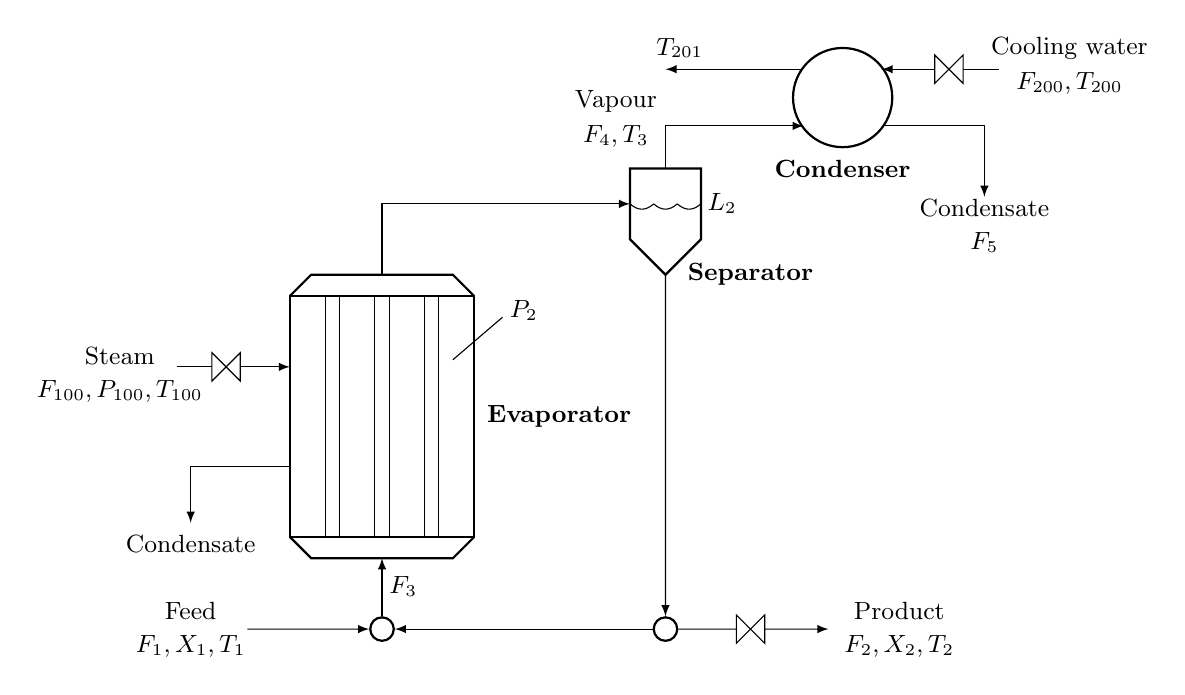
\begin{tikzpicture}[scale=0.9]

	% Evaporator
	\draw[thick] (-1.3,-1.7) rectangle (1.3, 1.7);
	\draw[thick] (-1.3,1.7) -- (-1.0, 2) -- (1.0, 2) -- (1.3, 1.7);
	\draw[thick] (-1.3,-1.7) -- (-1.0, -2) -- (1.0, -2) -- (1.3, -1.7);
	\draw (-0.1,-1.7) rectangle (0.1,1.7);
	\draw (-0.8,-1.7) rectangle (-0.6,1.7);
	\draw (0.6,-1.7) rectangle (0.8,1.7);
	\node at (2.5,0) {\bf \small Evaporator};
	\path[line] (0,2) |- (3.5,3);
	\path[line] (-1.3,-0.7) -| (-2.7,-1.5);
	\path[line] (-2.9,0.7) -- (-1.3,0.7);
	\node at (0.3,-2.4){\small $F_3$};
	\node at (2.0,1.5){\small $P_2$}; \draw (1.7,1.4) -- (1.0,0.8);
	\node at (-2.7,-1.8){\small Condensate};
	\node at (-2.7,-2.75){\small Feed}; \node at (-2.7,-3.25){\small $F_1, X_1, T_1$};
	\node at (-3.7,0.85){\small Steam}; \node at (-3.7,0.35){\small $F_{100},P_{100},T_{100}$}; %\node at (-3.5,0.2){\small $T_{100}$};
	
	\draw[fill=white] (-2.4,0.5) -- (-2.0,0.9) -- (-2.0,0.5) -- (-2.4,0.9) -- cycle;
	
	
	% Bottom
	\node at (0,-3) [dot, inner sep=3pt](dot1){};
	\node at (4,-3) [dot, inner sep=3pt](dot2){};
	\path[line] (dot2.west) -- (dot1.east);
	\path[line] (dot2.east) -- (6.3,-3);
	\path[line] (-1.9,-3) -- (dot1.west);
	\path[line] (dot1.north) -- (0,-2);
	\node at (7.3,-2.75){\small Product}; \node at (7.3,-3.25){\small $F_2, X_2, T_2$};
	
	\draw[fill=white] (5,-3.2) -- (5.4,-2.8) -- (5.4,-3.2) -- (5,-2.8) -- cycle;
	
	% Separator
	\draw[thick] (4,2) -- (3.5,2.5) -- (3.5,3.5) -- (4.5,3.5) -- (4.5,2.5) -- cycle;
	\node at (5.2,2) {\bf \small Separator};
	\path[line] (4,2) -- (dot2.north);
	\path[line] (4,3.5) |- (5.95,4.1);
	\node at (4.8,3){\small $L_2$};
	\node at (3.3,4.45){\small Vapour}; \node at (3.3,3.95){\small $F_4,T_3$};
	\node at (4.2,5.2){\small $T_{201}$};
	\draw (3.5,3) .. controls (3.61111,2.9) and (3.72222,2.9) .. (3.83333,3);
	\draw (3.83333,3) .. controls (3.944444,2.9) and (4.055555,2.9) .. (4.166666,3);
	\draw (4.166666,3) .. controls (4.277777,2.9) and (4.388888,2.9) .. (4.5,3);
	
	% Condenser
	\draw[thick] (6.5,4.5) circle (.7cm);
	\node at (6.5,3.5) {\bf \small Condenser};
	\path[line] (7.07,4.1) -| (8.5,3.1);
	\path[line] (8.7,4.9) -- (7.05,4.9);
	\path[line] (5.92,4.9) -- (4,4.9);
	\node at (9.7,5.20){\small Cooling water}; \node at (9.7,4.70){\small $F_{200},T_{200}$};
	\node at (8.5,2.95){\small Condensate}; \node at (8.5,2.45){\small $F_5$};
	
	\draw[fill=white] (7.8,4.7) -- (8.2,5.1) -- (8.2,4.7) -- (7.8,5.1) -- cycle;

\end{tikzpicture}
\caption{\small Schematic of the forced-circulation evaporator model of \cite{NeLe89}. The model consists of three distinct components: the evaporator, separator and condenser. The state of the system is made up of the product composition $X_2$, the evaporator pressure $P_2$ and the separator level $L_2$. The controlled inputs are product flow rate $F_2$, steam pressure $P_{100}$ and the cooling water flow rate $F_{200}$ which are applied through servomechanisms.}
\label{fig:evap}
\end{figure}
% ----------------------------------------------------



\subsection{Linear Control Theory}
\subsubsection{Model Identification}
The derivation of the nonlinear equations of motion of the system given in \App{evaporator} requires a reasonably detailed understanding of the physics involved in the process, including mass and energy balance equations. It also requires significant understanding of the system to know whether these equations will capture all the salient features of the actual plant. However, once we have this model it will be relatively easy to tune any uncertain parameters, such as physical constants, from observed data.


An alternative to using this first principles nonlinear model is to use techniques from System Identification. The vast majority of these methods focus on the identification of linear systems and address problems such as how to obtain a sufficiently rich training data set from a system operating in closed loop. The simplest example is the \textit{step-test} procedure, in which the tranfer function between each action and state is assumed to be first (or second) order and the parameters are directly estimated from the associated step responses. This makes very strict assumptions on the form of the dynamics but can often provide a model that is good enough for control design. More sophisticated techniques, such as \textit{subspace methods}, learn the parameters of a linear state-space model directly. For an accessible introduction to System Identification we direct the reader to the text by \cite{Lju99}.
 

One of the issues with identifying a linear model is how to ensure that the data we use for identification comes from a linear regime of the system. In many applications the nonlinearities are not aggressive enough to cause too much concern. A potential solution is to first fit a general nonlinear model to the data then linearise the model. However, it is generally an easier problem to confront the issues of obtaining a linear data set than to face the ones involved in choosing an appropriate nonlinear model. This issue could be alleviated through the use of a nonparametric modelling method such as Gaussian processes.


If we were to consider the modelling process from the very beginning, a major question is: how do we actually choose an appropriate representation of the state-space that will capture all the relevant features of the system?
%
The choice of $X_2$, $P_2$ and $L_2$ came from the expert knowledge used to derive the first principles model outlined in \App{evaporator}. However, this may not be a full enough representation in real life. For example, if we consider the fact that the actions will be applied through some servomechanisms with dynamics of their own it will be necessary to augment the state space to take account of this. Now, assuming we do have a sufficient state-representation and a model we can move onto the design of a control policy.


\subsubsection{Control Policy Design}
A common approach to controller design in industry is to split the multivariable loop into Single Input Single Output (SISO) loops by assigning each control action to one of the states. There are then many techniques available for tuning each individual feedback loop, for example PID controllers tuned using the Zeigler-Nichols rules. In reality, it may be very difficult to isolate such loops and there will, almost certainly, be coupling between each loop, the effect of which will have to be accounted for in a heuristic manner. \cite{NeLe89} discuss a method of achieving this for the evaporator. A fairly clear choice of SISO loops for the evaporator would be to control the separator level $L_2$ with the product flow rate $F_2$, the evaporator pressure $P_2$ with the input steam pressure $P_{100}$ and the product composition $X_2$ with the cooling water flow rate $F_{200}$. This choice could be obtained by looking at the physical system process in \Fig{evap}. Thus begins an iterative procedure of closing the feedback loop on each pair in turn then returning to the first one and repeating the process.


Applying a multivariable control design technique, such as LQR, circumvents the above issues. Standard LQR provides only proportional feedback terms and therefore cannot guarantee offset free setpoint tracking. To address this, we can explicitly incorporate integral action into the LQ tracking problem using the augmented dynamics trick by defining the state-space system
\begin{equation}
\bmat{\bx^{\bx}_{k+1} \\ \bx^{\br}_{k+1} \\ \bx^{\bee}_{k+1}} = 
\bmat{\bA & \bO & \bO \\ \bO & \bA^{\br} & \bO \\ \bC & -\bC^{\br} & \bI}
\bmat{\bx^{\bx}_{k} \\ \bx^{\br}_{k} \\ \bx^{\bee}_{k}}
+ \bmat{\bB \\ \bO \\ \bO}\bu_k
\label{eqn:evap_aug}
\end{equation}
where $\bx^{\bx}$ is the system state, $\bx^{\br}$ is the reference state and $\bx^{\bee}$ is integral of the error $\bC\bx^{\bx} - \bC^{\br}\bx^{\br}$. The integral of the error can be written in discrete-time as
\begin{equation*}
\bx^{\bee}_{k} = \sum_{i=0}^k  \bC\bx^{\bx}_i - \bC^{\br}\bx^{\br}_i
\end{equation*}
If we consider the tracking of a fixed state setpoint then $\bA^{\br} = \bC^{\br} = \bC = \bI$ and the elements of $\bx^{\br}$ contain the setpoints of the relevant state variables. We can then solve a standard LQR problem in this augmented state.
%
This approach effectively introduces a new set of integral terms which will help acheive offset-free tracking. \cite{NeLe89} report a significant performance improvement of this method over the standard SISO PID loops, even with na\"{\i}vely chosen state and action weighting matrices. 


These local control laws may only provide good performance in the region of the state space in which the linearised model was obtained. Therefore we need to address the issue of changing setpoint values that take us into regions of the state space where this model is no longer useful. This issue is traditionally addressed through the use of Gain Scheduling. A number of linear control laws are designed for different setpoint values, then a heuristic smoothing scheme is designed to switch between them. Alternatively, one could use a known nonlinear model online to obtain linearised models based on where we are in the state space. The control actions could then be determined using, for example, an LQR or MPC scheme.




\subsection{Learning Control}
\subsubsection{Problem Setup}
We now attack this problem from a learning control perspective. Assuming that we have some representation of the state, and have been given a set of control actions we need to design an appropriate prior over system dynamics $p(\bff)$, stage-cost $c(\cdot)$ and policy structure $\bpi(\cdot)$. We shall talk about each one of these considerations in turn.
%
We note that, as in the previous section, a major issue with tackling this problem using minimal expert knowledge is how to actually choose an appropriate representation for the state. In this case, there is no obvious reasoning to choose $X_2, P_2$ and $L_2$ without a reasonable understanding of the physics of the problem. Therefore, we shall assume that this state representation is given.

%The reasoning to have $X_2, P_2$ and $L_2$ as part of the control objective is
%\begin{itemize}
%\item
%The overall aim of this process is to control the product composition $X_2$
%\item
%The pressure in the evaporator $P_2$ and the level of the separator $L_2$ must be kept within hard constraints
%\end{itemize}
%However, . A more rigorous line of reasoning would require a deeper level of insight into the problem which we will not go into here.



\subsubsection{Prior Over Dynamics}
We choose a completely general squared-exponential prior over the unknown dynamics. We can achieve reference tracking and controller integral action using the framework of augmented dynamics outlined in Chapter 3 and in a similar spirit to \Eq{evap_aug}. We will use the following sub-dynamics models
\begin{align*}
\bx^{\bx}_{k+1} &= \bff_1\big(\bx^{\bx}_{k}, \bu_k \big)
 \sim \mathcal{GP}(\bO,\bK_{\te{SE}}) \\
\bx^{\br}_{k+1} &= \bff_2\big(\bx^{\br}_{k} \big)
= \bA^{\br} \bx^{\br}_{k} \\
\bx^{\bee}_{k+1} &= \bff_3\big(\bx^{\bx}_{k},\bx^{\br}_{k},\bx^{\bee}_{k} \big) 
= (\bC\bx^{\bx}_{k} - \bC^{\br}\bx^{\br}_{k}) + \bx^{\bee}_{k} 
\end{align*}
where we learn the main system dynamics with a Gaussian process, we will define an appropriate linear model for the reference state and the integral of the error is simply another linear relationship. If we consider reference tracking on $X_2$ and $P_2$ only then $\bC = [\bI,\bO] \in \RR^{2\times 3}$.

We could also encode an approximating linear model for the servomechanisms by adding a fourth sub-dynamics and altering the first as follows
\begin{align*}
\bx^{\bx}_{k+1} &= \bff_1\big(\bx^{\bx}_{k}, \bx^{\bu}_{k}, \bu_k \big)
\sim \mathcal{GP}(\bO,\bK_{\te{SE}}) \\
\bx^{\bu}_{k+1} &= \bff_4\big( \bx^{\bu}_{k}, \bu_k \big)
= a\bx^{\bu}_k + (1 - a)\bu_k
\end{align*}
where $a = \mathrm{exp}(-\Dt/\tau_u)$, $\tau_u$ is our approximate time lag, $\bx^{\bu}$ is that action actually applied to the system through the servomechanism and $\bu$ is now the input to the servo itself. Clearly as $\tau_u \rightarrow 0$ the dependence of $\bff_1$ on $\bx^{\bu}$ will decrease and it will be reasonable to simply ignore its effect.





\subsubsection{Stage-Cost Function}
We shall split our stage-cost into two parts $c(\bx) = c_1(\bx) + c_2(\bx)$. The first penalises deviations from the $X_2$ and $P_2$ setpoints. We use the inverted-Gaussian stage-cost from \Eq{cost_gauss} where $\bQ$ is chosen such that the one-standard deviation limits are $\pm 10\%$ on $X_2$ and $\pm 20\,$kPa on $P_2$, with respect to the given setpoint values. This is because we do not expect to be operating more than $\pm 20\%$ or $40\,$kPa from a given setpoint and therefore this is an appropriate metric for choosing the ``2$\sigma$ region" of our cost.
Deviation from the $L_2$ setpoint is not explicitly penalised since we only really care that the level stays within its limits.


The second part of the cost accounts for the constraints on $P_2$ and $L_2$. For this we use the affine cost given in \Eq{con_aff} with slopes of $10\,$kPa per unit cost on $P_2$ and $0.1\,$m per unit cost on $L_2$ in the constraint violation regions. We are aiming to keep them within $P_2 \in [0,100]\,$kPa and $L_2\in [0,4]\,$m therefore the corners of the affine regions will be placed at these locations. A more cautious approach would place the corners on the interior of these regions. An example of this cost function is shown in \Fig{bazza} where we can see that the policy should adopt cautious behaviour when acting close to the state boundaries. In other words, it should only operate close to a state boundary if it is certain of the state trajectory that will be taken.




%-------------------------------------------------------------------------------------------------------------------------------------------
\begin{figure}
\centering
\tikzstyle{line} = [draw, -latex]
\begin{tikzpicture}
\small
\node at (0,0) {\includegraphics[scale=0.6,clip,trim=0.3cm 0.4cm 0cm 0cm]{figs/comp/barrier.pdf}};
\node at (0,-2.9) {Constrained state};
\node at (-3.15,1.15) {$c(x)$};
\node at (3,-2.8) {$x_{\te{max}}$};
\node at (-3,-2.8) {$x_{\te{min}}$};
\node[rotate=90] at (-5.2,0) {Barrier cost};
\node at (0.9,-0.3) {\color{blue}$p_1(x)$};
\node at (-0.2,-1.9) {\color{red}$p_2(x)$};
\end{tikzpicture}
\caption{Illustration of the intrinsic caution introduced when using barrier functions as soft constraints. Note that $p_2(x)$ will be penalised more heavily than $p_1(x)$ even though its mean is further away from the constraint edge.}
\label{fig:bazza}
\end{figure}
%-------------------------------------------------------------------------------------------------------------------------------------------










\subsubsection{Policy Structure}
We shall consider an affine policy structure. This will not have access to a preview horizon of the reference and therefore is a function of $\bx^{\bx}, \bC^{\br}\bx^{\br}$ and $\bx^{\bee}$ to allow for the possibility of integral action. Since we will only be tracking setpoints on $X_2$ and $P_2$ we only require a reference and integral action on these dimensions therefore our policy will have to map seven state variables (the three system states, two reference states and two integral states) to the three action variables.

We note that for this application an affine policy may not be flexible enough to track setpoints across a variety of regions in the state space. In the situations where a linear policy is not sufficient we could use a general Radial Basis Function (RBF) policy. However, this may be unnecessarily flexible and requires basis functions spread across the whole state space. In our seven dimensional input space this would require $n_c = 10^7$ basis functions just to provide a grid of 10 points in each dimension. An alternative class of functions which does not suffer from the same curse of dimensionality is the family of additive RBFs. An example of a single output first order additive Gaussian-RBF is
\begin{equation}
\pi(\bx) = \sum_{i=1}^{n_c} w_i \sum_{d=1}^{E} \alpha_{d}^2
\exp\Big( \tfrac{1}{2} \big(x[d] - \mu_{i}[d]\big)^2/\lambda_d^2 \Big)
\end{equation}
with $n_c$ basis functions each with individual weights $w_i$ and centres $\bm_i$.
These functions can are of the general form $\bpi(\bx) = \bpi_1\big(x[1]\big) + \dots + \bpi_E\big(x[E]\big)$ and are therefore more flexible than affine policies but more restricted than a general RBF. In this case we only have to provide basis functions along a single dimensional subspace. In our example, the ten dimensional grid could be achieved with only ten basis functions!


%-------------------------------------------------------------------------------------------------------------------------------------------
\begin{figure}[t]
\centering \footnotesize
\subfigure[RBF]{
\begin{tikzpicture}
  \node at (0,0) {\includegraphics[scale = 0.6, clip, trim=0.45cm 0.4cm 0cm 0cm]{figs/comp/rbf.pdf}};
\end{tikzpicture}
\label{fig:RBFfig}
}
\subfigure[Additive RBF]{
\begin{tikzpicture}
  \node at (0,0) {\includegraphics[scale = 0.6, clip, trim=0.45cm 0.4cm 0cm 0cm]{figs/comp/rbfa.pdf}};
\end{tikzpicture}
\label{fig:aRBFfig}
}
\caption{Basis function locations to provide a grid over a two dimensional space for a standard RBF compared with an additive RBF.}
\label{fig:RBFs}
\end{figure}
%-------------------------------------------------------------------------------------------------------------------------------------------





\subsubsection{Safe Implementation}
A further consideration due to the nature of the problem is that during the learning phase we cannot allow the system to ``crash"! To address this issue we will assume that there is a working control policy (possibly a human operator) already on the plant from which we can obtain an initial training data set and can hand control back to during the learning phase. We will have to define, in a heuristic manner, boundaries on the states and actions which, if violated, the system will hand control back to the original control policy. Learning can then proceed in a safe manner, provided that the original control policy can react fast enough to recover the system from the boundary of the violation.





\subsection{Application of Learning Control}
\subsubsection{Experimental Setup}

We now set out to implement learning control on a simulated model of the evaporator. The simulated model was based on the equations defined in \App{evaporator} with the controlled inputs applied through servomechanisms modelled as first-order lags with time constant $\tau_u$. We limited the number of function evaluations in the policy optimisation stage to 50 in order to place a limit on the computation time.

Our task will be to design a control policy to track a number of possible setpoint changes on $X_2$ and $P_2$. The setpoint change for $X_2$ will be from $\cN(25,0.5^2)$ to $\cN(15,2^2)$ each sampled independently. Similarly the change on $P_2$ will be from $\cN(50,1^2)$ to $\cN(70,5^2)$. The change will take place linearly over a period of 5 mins. These setpoint changes are shown in \Fig{X2P2sets}. The reference state space model we use to achieve this, for $X_2$ for example, is
\begin{align*}
\bx^{\br}_{k+1} = \underbrace{ \bmat{\bO & \bI \\ 0 & \bmat{\bO & 1}} }_{\bA^{\br}}   \bx^{\br}_{k}
\quad\text{and}\quad
X_{2,k}^r = \underbrace{ \bmat{1 & \bO}  }_{\bC^{\br}}   \bx^{\br}_{k}
\end{align*}
with the following choice of distribution over $\bx^{\br}_{0}$ to obtain the 5 minute transitioning regime shown in \Fig{X2fig}
\begin{equation}
\bx^{\br}_{0} \sim \cN\left(
\bmat{\balp & (\mathbf{1}-\balp)}\bmat{25 \\ 15},
\bmat{\balp & (\mathbf{1}-\balp)} \bmat{0.5^2 & 0 \\ 0 & 2^2} \bmat{\balp\T \\ (\mathbf{1}-\balp)\T}
\right)
\end{equation}
where $\balp = [1,1,1,1,1,1,0.8,0.6,0.4,0.2,0]\T \in \RR^{11}$. A similar process is then carried out for $P_2$.






%-------------------------------------------------------------------------------------------------------------------------------------------
\begin{figure}[t]
\centering \footnotesize
\subfigure[$X_2$ setpoint]{
\begin{tikzpicture}
  \node at (0,0) {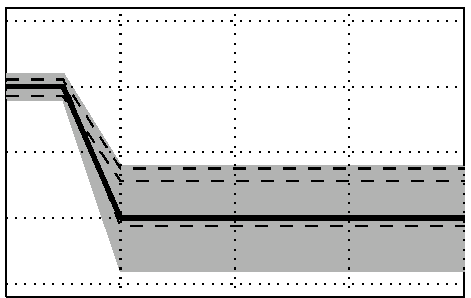
\includegraphics[scale = 0.8]{figs/comp/set_X2.pdf}};
  \node at (0.1,-2.35) {time (mins)};
  \node at (-3.1,-2.3) {0};  \node at (3.1,-2.3) {40};
  \node[rotate=90] at (-3.4,0) {$X_2$ (\%)};
  \node at (-3.4,1.75) {30}; \node at (-3.4,-1.8) {10};
\end{tikzpicture}
\label{fig:X2fig}
} \hfill
\subfigure[$P_2$ setpoint]{
\begin{tikzpicture}
  \node at (0,0) {\includegraphics[scale = 0.8]{figs/comp/set_P2.pdf}};
  \node at (0.1,-2.35) {time (mins)};
  \node at (-3.1,-2.3) {0};  \node at (3.1,-2.3) {40};
  \node[rotate=90] at (-3.4,0) {$P_2$ (kPa)};
  \node at (-3.4,1.75) {80}; \node at (-3.4,-1.8) {40};
\end{tikzpicture}
\label{fig:P2fig}
}
\caption{Distributions over possible setpoint changes for the states $X_2$ and $P_2$. The change takes place over a period of 5 mins using a ramp function. The thick black line depicts the mean of the change, the gray areas denotes the 2$\sigma$ region and samples from these distributions are given by dashed lines.}
\label{fig:X2P2sets}
\end{figure}
%-------------------------------------------------------------------------------------------------------------------------------------------




%-------------------------------------------------------------------------------------------------------------------------------------------
\begin{figure}[]
\centering \footnotesize
\subfigure[Affine control policy]{
\begin{tikzpicture}
	\foreach \x / \i in {0/1, 2.8/2, 5.6/3, 8.4/4, 12.5/6} {
		\node at (\x,2.8) {\includegraphics[scale=0.8]{figs/comp/affine_X\i.pdf}};
		\node at (\x,0) {\includegraphics[scale=0.8]{figs/comp/affine_P\i.pdf}};
		\node at (\x,-2.8) {\includegraphics[scale=0.8]{figs/comp/affine_L\i.pdf}};
		\node at (\x,-4.35) {Trial \i};
	}
	\node at (10.45,2.8) {$\dots$}; \node at (10.45,0) {$\dots$}; \node at (10.45,-2.8) {$\dots$};
	\node[rotate=90] at (-1.5,2.8) {\small composition $X_2$};
	\node[rotate=90] at (-1.5,0) {\small pressure $P_2$};
	\node[rotate=90] at (-1.5,-2.8) {\small tank level $L_2$};
\end{tikzpicture}
\label{fig:pol_aff}
}
\subfigure[Additive Gaussian-RBF control policy]{
\begin{tikzpicture}
	\foreach \x / \i in {0/1, 2.8/2, 5.6/3, 9.7/5, 12.5/6} {
		\node at (\x,2.8) {\includegraphics[scale=0.8]{figs/comp/additive_X\i.pdf}};
		\node at (\x,0) {\includegraphics[scale=0.8]{figs/comp/additive_P\i.pdf}};
		\node at (\x,-2.8) {\includegraphics[scale=0.8]{figs/comp/additive_L\i.pdf}};
		\node at (\x,-4.35) {Trial \i};
	}
	\node at (7.65,2.8) {$\dots$}; \node at (7.65,0) {$\dots$}; \node at (7.65,-2.8) {$\dots$};
	\node[rotate=90] at (-1.5,2.8) {\small composition $X_2$};
	\node[rotate=90] at (-1.5,0) {\small pressure $P_2$};
	\node[rotate=90] at (-1.5,-2.8) {\small tank level $L_2$};
\end{tikzpicture}
\label{fig:pol_add}
}
\caption{Trajectories of the state variables of the evaporator over five independent runs of the learning algorithm using different policy structures. The trials are the application of the current best policy after a given simulation phase. The actual state trajectories are given in blue, the setpoints are given in red and the tank constraints are given by the red dashed lines. The x-axes depict a range of $[0, 40]\,$mins while the y-axes show $[10, 30]\,$\%, $[40, 80]\,$kPa and $[-0.2, 4.2]\,$m for $X_2$, $P_2$ and $L_2$ respectively.}
\label{fig:randy}
\end{figure}
%-------------------------------------------------------------------------------------------------------------------------------------------



\subsubsection{Altering the Policy Structure}
Our initial training data set was generated from a crudely designed LQR control policy for the equilibrium at $X_2 = 25\,$\% and $P_2 = 50.5\,$kPa. The training data set consisted of two 20 minute trajectories showing this control policy regulating the system back to its setpoint from an initial perturbation of $X_2 \sim \cN(25,2^2)$ and $P_2 \sim \cN(50,5^2)$. The simulation stage of the algorithm then aimed to minimise a cost function over a horizon of 40 minutes and using the stage cost outlined in the previous section.


The first set of experiments we ran was on a system with servomechanism time constants of $\tau_u = 0.1\,$mins. In this case we ignore the additional states introduced by the lags and use only the normal system states and control actions for modelling. We compare the results of using an affine feedback policy and an additive Gaussian-RBF policy with a grid of 30 basis functions in the region of operation. The affine policy therefore has a total of 24 free parameters. For the Gaussian-RBF we fix the centres of each basis function but leave the length scales, output scales and weights to be tuned automatically, a total of 132 free parameters. Each policy has access to the integral of the error between the setpoints on $X_2$ and $P_2$ and their actual location, therefore are able to achieve integral action.


The results of the simulation we have just described are given in \Fig{randy}. Let us first discuss the performance of the learned affine policy shown in \Fig{pol_aff}. We can observe in the trial of the first learned policy that some of the runs have found a solution that is stabilising but not yet able to track while others have completely failed and have to be stopped before they drain the separator tank. By the second trial most policies have stabilised the system but it is only by the fourth trial that offset-free tracking is achieved. This has taken a total of 2 hours of interaction (plus the initial training data set) to achieve this performance. 


We now turn our attention to the performance of the additive RBF policy given in \Fig{pol_add}. We can see that by the third iteration it has stabilised all the runs, in contrast to the affine policy which took until the fourth. However, it actually takes the policy until the sixth trial to exploit the integral action capability required to achieve offset free tracking as can be clearly observed when comparing the results at the fifth and sixth trials. The reason for this slow learning is most likely the fact that we restrict the policy optimisation to only 50 function evaluations. The decrease in cost when moving from a simply stabilising to a tracking policy is relatively small but the change in policy parameters may be large, therefore the 50 evaluations was not enough to actually reach the optimal solution after a given trial.

We further note that it may appear from the plots in \Fig{randy} that the policy has access to some preview horizon of the setpoint change as it appears to anticipate the change. This is actually not the case and is simply because neither policy has learned, or is able, to apply offset free tracking at both setpoints.




%-------------------------------------------------------------------------------------------------------------------------------------------
\begin{figure}[]
\centering \footnotesize
\subfigure[Assumed servomechanism lag of 0.8$\,$mins]{
\begin{tikzpicture}
	\foreach \x / \i in {0/1, 2.8/2, 5.6/3, 8.4/4, 12.5/8} {
		\node at (\x,2.8) {\includegraphics[scale=0.8]{figs/comp/lag08_X\i.pdf}};
		\node at (\x,0) {\includegraphics[scale=0.8]{figs/comp/lag08_P\i.pdf}};
		\node at (\x,-2.8) {\includegraphics[scale=0.8]{figs/comp/lag08_L\i.pdf}};
		\node at (\x,-4.35) {Trial \i};
	}
	\node at (10.45,2.8) {$\dots$}; \node at (10.45,0) {$\dots$}; \node at (10.45,-2.8) {$\dots$};
	\node[rotate=90] at (-1.5,2.8) {\small composition $X_2$};
	\node[rotate=90] at (-1.5,0) {\small pressure $P_2$};
	\node[rotate=90] at (-1.5,-2.8) {\small tank level $L_2$};
\end{tikzpicture}
\label{fig:lag08}
}
\subfigure[Assumed servomechanism lag of 0.4$\,$mins]{
\begin{tikzpicture}
	\foreach \x / \i in {0/1, 2.8/2, 6.25/4, 9.05/5, 12.5/8} {
		\node at (\x,2.8) {\includegraphics[scale=0.8]{figs/comp/lag04_X\i.pdf}};
		\node at (\x,0) {\includegraphics[scale=0.8]{figs/comp/lag04_P\i.pdf}};
		\node at (\x,-2.8) {\includegraphics[scale=0.8]{figs/comp/lag04_L\i.pdf}};
		\node at (\x,-4.35) {Trial \i};
	}
	\node at (10.78,2.8) {$\dots$}; \node at (10.78,0) {$\dots$}; \node at (10.78,-2.8) {$\dots$};
	\node at (4.55,2.8) {$\dots$}; \node at (4.55,0) {$\dots$}; \node at (4.55,-2.8) {$\dots$};
	\node[rotate=90] at (-1.5,2.8) {\small composition $X_2$};
	\node[rotate=90] at (-1.5,0) {\small pressure $P_2$};
	\node[rotate=90] at (-1.5,-2.8) {\small tank level $L_2$};
\end{tikzpicture}
\label{fig:lag04}
}
\caption{Trajectories of the state variables of the evaporator over five independent runs of the learning algorithm where wrong approximations of the real servomechanism lag of 1.2$\,$mins are forced upon the internal model of the dynamics. The trials are the application of the current best policy after a given simulation phase. The actual state trajectories are given in blue, the setpoints are given in red and the tank constraints are given by the red dashed lines. The x-axes depict a range of $[0, 40]\,$mins while the y-axes show $[10, 30]\,$\%, $[40, 80]\,$kPa and $[-0.2, 4.2]\,$m for $X_2$, $P_2$ and $L_2$ respectively.}
\label{fig:laggy}
\end{figure}
%-------------------------------------------------------------------------------------------------------------------------------------------



\subsubsection{Incorporating Erroneous Prior Information}

The second set of experiments we ran involved learning to track a deterministic setpoint change, given by the means in \Fig{X2P2sets}. The use of a deterministic change is simply to make our plots clearer. For these experiments we use the full nonlinear system of equations with control actions applied through servomechanisms with lags of $\tau_u=1.2\,$mins, as used by \cite{Mac02}. The problem we investigate is the effect of incorporating erroneous prior information into the model of the system, in this case: a model for the servomechanisms with an underestimated value of $\tau_u$. 


The results for a wrongly modelled lag of $\tau_u=0.8\,$mins (a mismatch of 33$\,$\%) are shown in \Fig{lag08} and the results for $\tau_u=0.4\,$mins (a mismatch of 66$\,$\%) are in \Fig{lag04}. It is clear from \Fig{lag08} that a discrepancy of 33$\,$\% causes little disruption to the learning process aside from some unwanted oscillatory behaviour exhibited in the second and third trials. We note that an important issue with finite horizon trajectory optimisation is shown in trial eight. We see that one of the runs is rapidly approaching the upper constraint boundary and therefore incurs no penalty over the horizon. However, this is undesirable since obviously if we run it for any longer the constraint will be violated. This issue could be addressed by adding an additional penalty on $L_2$ penalising deviations from the 2$\,$m mark. Also, considering distributions over possible setpoint changes tends to deal with this issue.

We now turn our attention to a discrepancy of 66$\,$\% as in \Fig{lag04}. We can see that it has a strongly adverse effect on learning. Even so, by the eighth trial we can observe that three of the runs have managed to achieve the task with the other two getting close.
%
We further note that the learning process exhibits a useful feature. By trial four the algorithm has learned to satisfy the system constraints, which obviously is a more important criteria than the setpoint tracking itself. Once it has achieved this it starts to make improvements on the tracking performance as shown in trial five.








\section{Summary}
We have considered in this chapter various issues associated with control policy design from a classical perspective and from the learning control perspective that has been the subject of most of this thesis. The comparison was carried out in the context of two case studies: the unicycle and the evaporator. One of the main features of the classical control design that we drew out from the case studies was that often we have to deal with achievement of the task, satisfying system constraints and dealing with modelling mismatch all together with the cost function parameters. In other words, the solution to all these issues are coupled into the same design parameters. Methods such as MPC can separate out dealing with constraints but still require model mismatch and task achievement to be dealt with by the same tuning parameters. Conversely, in the learning algorithm, there are separate tuneable parameters associated with each problem and therefore tuning can take place in an arguably more intuitive manner.

Addressing the unicycle balancing problem specifically, we saw that it is actually a difficult problem just to obtain a linearised model appropriate for control design. This process actually requires significant knowledge of the underlying system dynamics. The learning algorithm can bypass this issue by using a learned nonlinear representation with little required expert knowledge. However, when comparing the learned control policy and an LQR control policy we find that the learned solution to the problem, although satisfying the cost criterion, will not be a good control policy in practice. This is because it converges on an orbital trajectory which will fall over once the time of the prediction horizon is over. 

Finally, the evaporator control problem threw up some interesting issues.  The first was the question of how to actually choose an appropriate state space representation of the system, which is necessary for both the classical and the learning methods. This process requires at least some high level intuition about the problem. We went on to show that the learning control method could be applied in a safe and intuitive manner to the problem with minimal tuning. In particular, we were able to train an additive Gaussian-RBF control policy to obtain greater generality than a standard affine structure but avoid the problem of choosing basis function locations common to standard RBFs. We also demonstrated that in this context the learning approach can handle significant modelling errors forced upon the dynamics prior. 


